% Author: Alfredo Sánchez Alberca (email:asalber@ceu.es)
% Plot with the phases of the statistical cycle
\begin{tikzpicture}[every label/.style={text=color1}]
\tikzstyle{arrow} = [-latex, color2, line width=12pt];
\tikzstyle{node} = [align=center, inner sep=10pt];
\node[node, label=-90:Population] (population) at (1,1)
{\includegraphics[height=1.5cm]{img/introduction/population}}; 
\pause
\node[node,label=90:Sample] (sample) at
(1,6){\includegraphics[height=1.5cm]{img/introduction/sample}}; 
\draw[arrow] (population) -- (sample) node[midway,rotate=90,white] {Sampling\quad\phantom{0}};
\pause
\node[node,label=90:Summary measures] (statistics) at (8,6) {\Large $\bar x$ \quad $s^2$\\\Large \quad $p$ \quad
$g_1$}; 
\draw[arrow] let \p1=(sample.east), \p2=(1,0) in (\x1+\x2,\y1) -- (statistics)
node[midway,white] {Descriptive\quad\phantom{0}}; 
\pause
\node[node,label=-90:Model] (model) at (8,1) {\includegraphics[scale=0.5]{img/introduction/model}};
\draw[arrow] (statistics) -- (model) node[midway,rotate=-90,white] {Inferential\quad\phantom{0}};
\pause
\draw[arrow] (model) -- (population) node[midway,white] {\quad Prediction};
\end{tikzpicture}